%! TEX root = ../main.tex
\documentclass[../main]{subfiles}

% ローカル下書き用
% \documentclass{supernova_pre}
% このクラスの中に大体のパッケージは入ってるので基本何でもかけるはず
% 追加したいパッケージがあればここに記入
\usepackage{multicol} % 3段組レイアウト用
\usepackage{enumitem} % 箇条書き調整用パッケージ

\begin{document}
\chapter{山で天文観測を楽しもう} % タイトル

\rightline{B3 森 章裕} % 学年と名前(ハンドルネームでも可)

\section{はじめに}
都市部での天体観測では、光害が大きな障害となります。都市の明かりによって空が明るくなり、星が見えづらくなってしまうからです。調布でも肉眼で見えるのは明るい惑星や3等星程度までです。

そこで快適な天体観測を行うために、光害の少ない山間部での天体観測を提案します。私はワンダーフォーゲル部にも所属しており、実際に合宿のキャンプ地で見れる星空は格別です。天文部でも山間部を合宿地として選ぶことが多いため、ぜひ皆さんも一緒に山に行きましょう。登山はいいぞ!

\section{山で天体観測するメリット}
山で天体観測を行うメリットは、光害が少ないという理由以外にもいくつかあります。

山の空気は都市に比べて澄んでいるので、星をより鮮明に見ることができます。また、山頂や尾根、高原などを観測場所に選ぶことによって広い視野を確保することができます。あと何よりも登山と天体観測が同時に楽しめるのがよいと思います。

\section{涸沢での観測}

9/25から9/27の日程で奥穂高に登るついでにキャンプ地の涸沢で天体観測をしてきました。その際の記録をまとめます。

\subsection{観測した場所}

\begin{figure}
\begin{minipage}{0.45\textwidth} % 左側(文章)の領域
  〒390-1520 長野県松本市安曇 涸沢野営場 \\

  涸沢はカールという氷河によって浸食された谷の中にあり、三方が山に囲まれているので低緯度の星は見えませんが、上高地方面の光が遮られるので星が見やすいと感じました。light pollution map\footnote{light pollution map, \url{https://www.lightpollutionmap.info/}}ではlight valueは0でした。
\end{minipage}%
\hfill
\begin{minipage}{0.45\textwidth} % 右側(画像)の領域
    \centering
    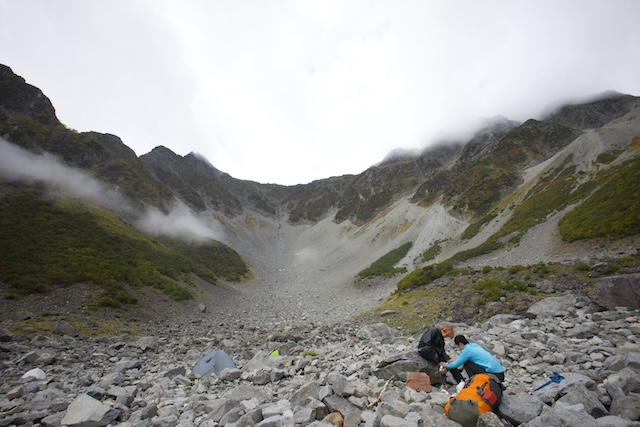
\includegraphics[width=\linewidth]{sections/mori/IMG_2413.jpg} % 画像のパスを指定
    \caption{涸沢キャンプ場}
\end{minipage}
\end{figure}

\subsection{行程}
【1日目】
\begin{quote}
  上高地バスターミナル(06:00)・・・河童橋(06:05)・・・明神(06:55)[休憩 10分]・・・徳沢(08:05)[休憩 10分]・・・横尾(09:25)[休憩 10分]・・・本谷橋(10:55)[休憩 10分]・・・涸沢(12:45)
\end{quote}

【2日目】
\begin{quote}
  涸沢(07:00)・・・ザイテングラート取付(08:40)[休憩 10分]・・・穂高岳山荘(09:50)[休憩 10分]・・・奥穂高岳(10:50)[休
  憩 20分]・・・穂高岳山荘(11:50)[休憩 20分]・・・ザイテングラート取付(12:55)[休憩 10分]・・・涸沢(14:05)
\end{quote}

【3日目】
\begin{quote}
  涸沢(07:00)・・・本谷橋(08:10)[休憩 10分]・・・横尾(09:10)[休憩 10分]・・・徳沢(10:30)[休憩 10分]・・・明神(11:40)[休憩 10分]・・・河童橋(12:40)[休憩 10分]・・・上高地バスターミナル(12:55)
\end{quote}


※上高地バスターミナルまでは新宿上高地間の夜行バスを利用

\subsection{準備した道具}

\subsubsection{登山用}
\begin{multicols}{3} % 3段組の環境を開始
  \begin{itemize}
    \item 半そでシャツ
    \item ズボン
    \item 登山靴
    \item 防寒着
    \item 靴下
    \item 手袋
    \item 着替えの予備
    \item 雨具
    \item 大型のザック
    \item 小型のザック
    \item ザックカバー
    \item シュラフ
    \item 寝袋マット
    \item テント
    \item ジェットボイル
    \item ガス
    \item 水筒2-4L分くらい
    \item ヘッドランプと予備電池
    \item 洗面用具
    \item 救急用品
    \item トイレットペーパー
    \item ジップロック
    \item 保険証
    \item 食料
    \item 行動食
    \item スマホ
    \item 現金
  \end{itemize}
\end{multicols}

\subsubsection{天体観測用}

\begin{itemize}
  \item (カメラ) EOS R100
  \item (レンズ) 銘匠光学 TTArtisan 10mm f/2 C ASPH.
  \item (三脚) Amazonベーシック 三脚 127cm
  \item (フィルター)スターエンハンサー 72mm
\end{itemize}

キャンプ場の涸沢まで6時間程度歩くため、観測用の機材は最低限にしました。三脚も山に持っていくことを考慮して安価で軽量なものを選択しました。観測用の機材で増えた重量は約1.5kg程度です。

\subsection{観測内容}
一日目は曇りで、翌日は奥穂高に登るので早く寝ました。
二日目は雲の流れが速かったですが、晴れている時間がかなりあったので9時まで観測しました。\\

\begin{figure}[H]
  \centering
  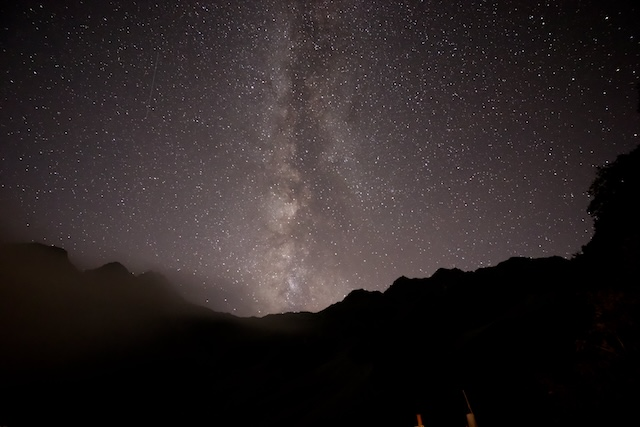
\includegraphics[width=0.7\linewidth]{sections/mori/IMG_2378.jpg}
  \caption{奥穂高岳と天の川}
\end{figure}

\begin{figure}[H]
  \centering
  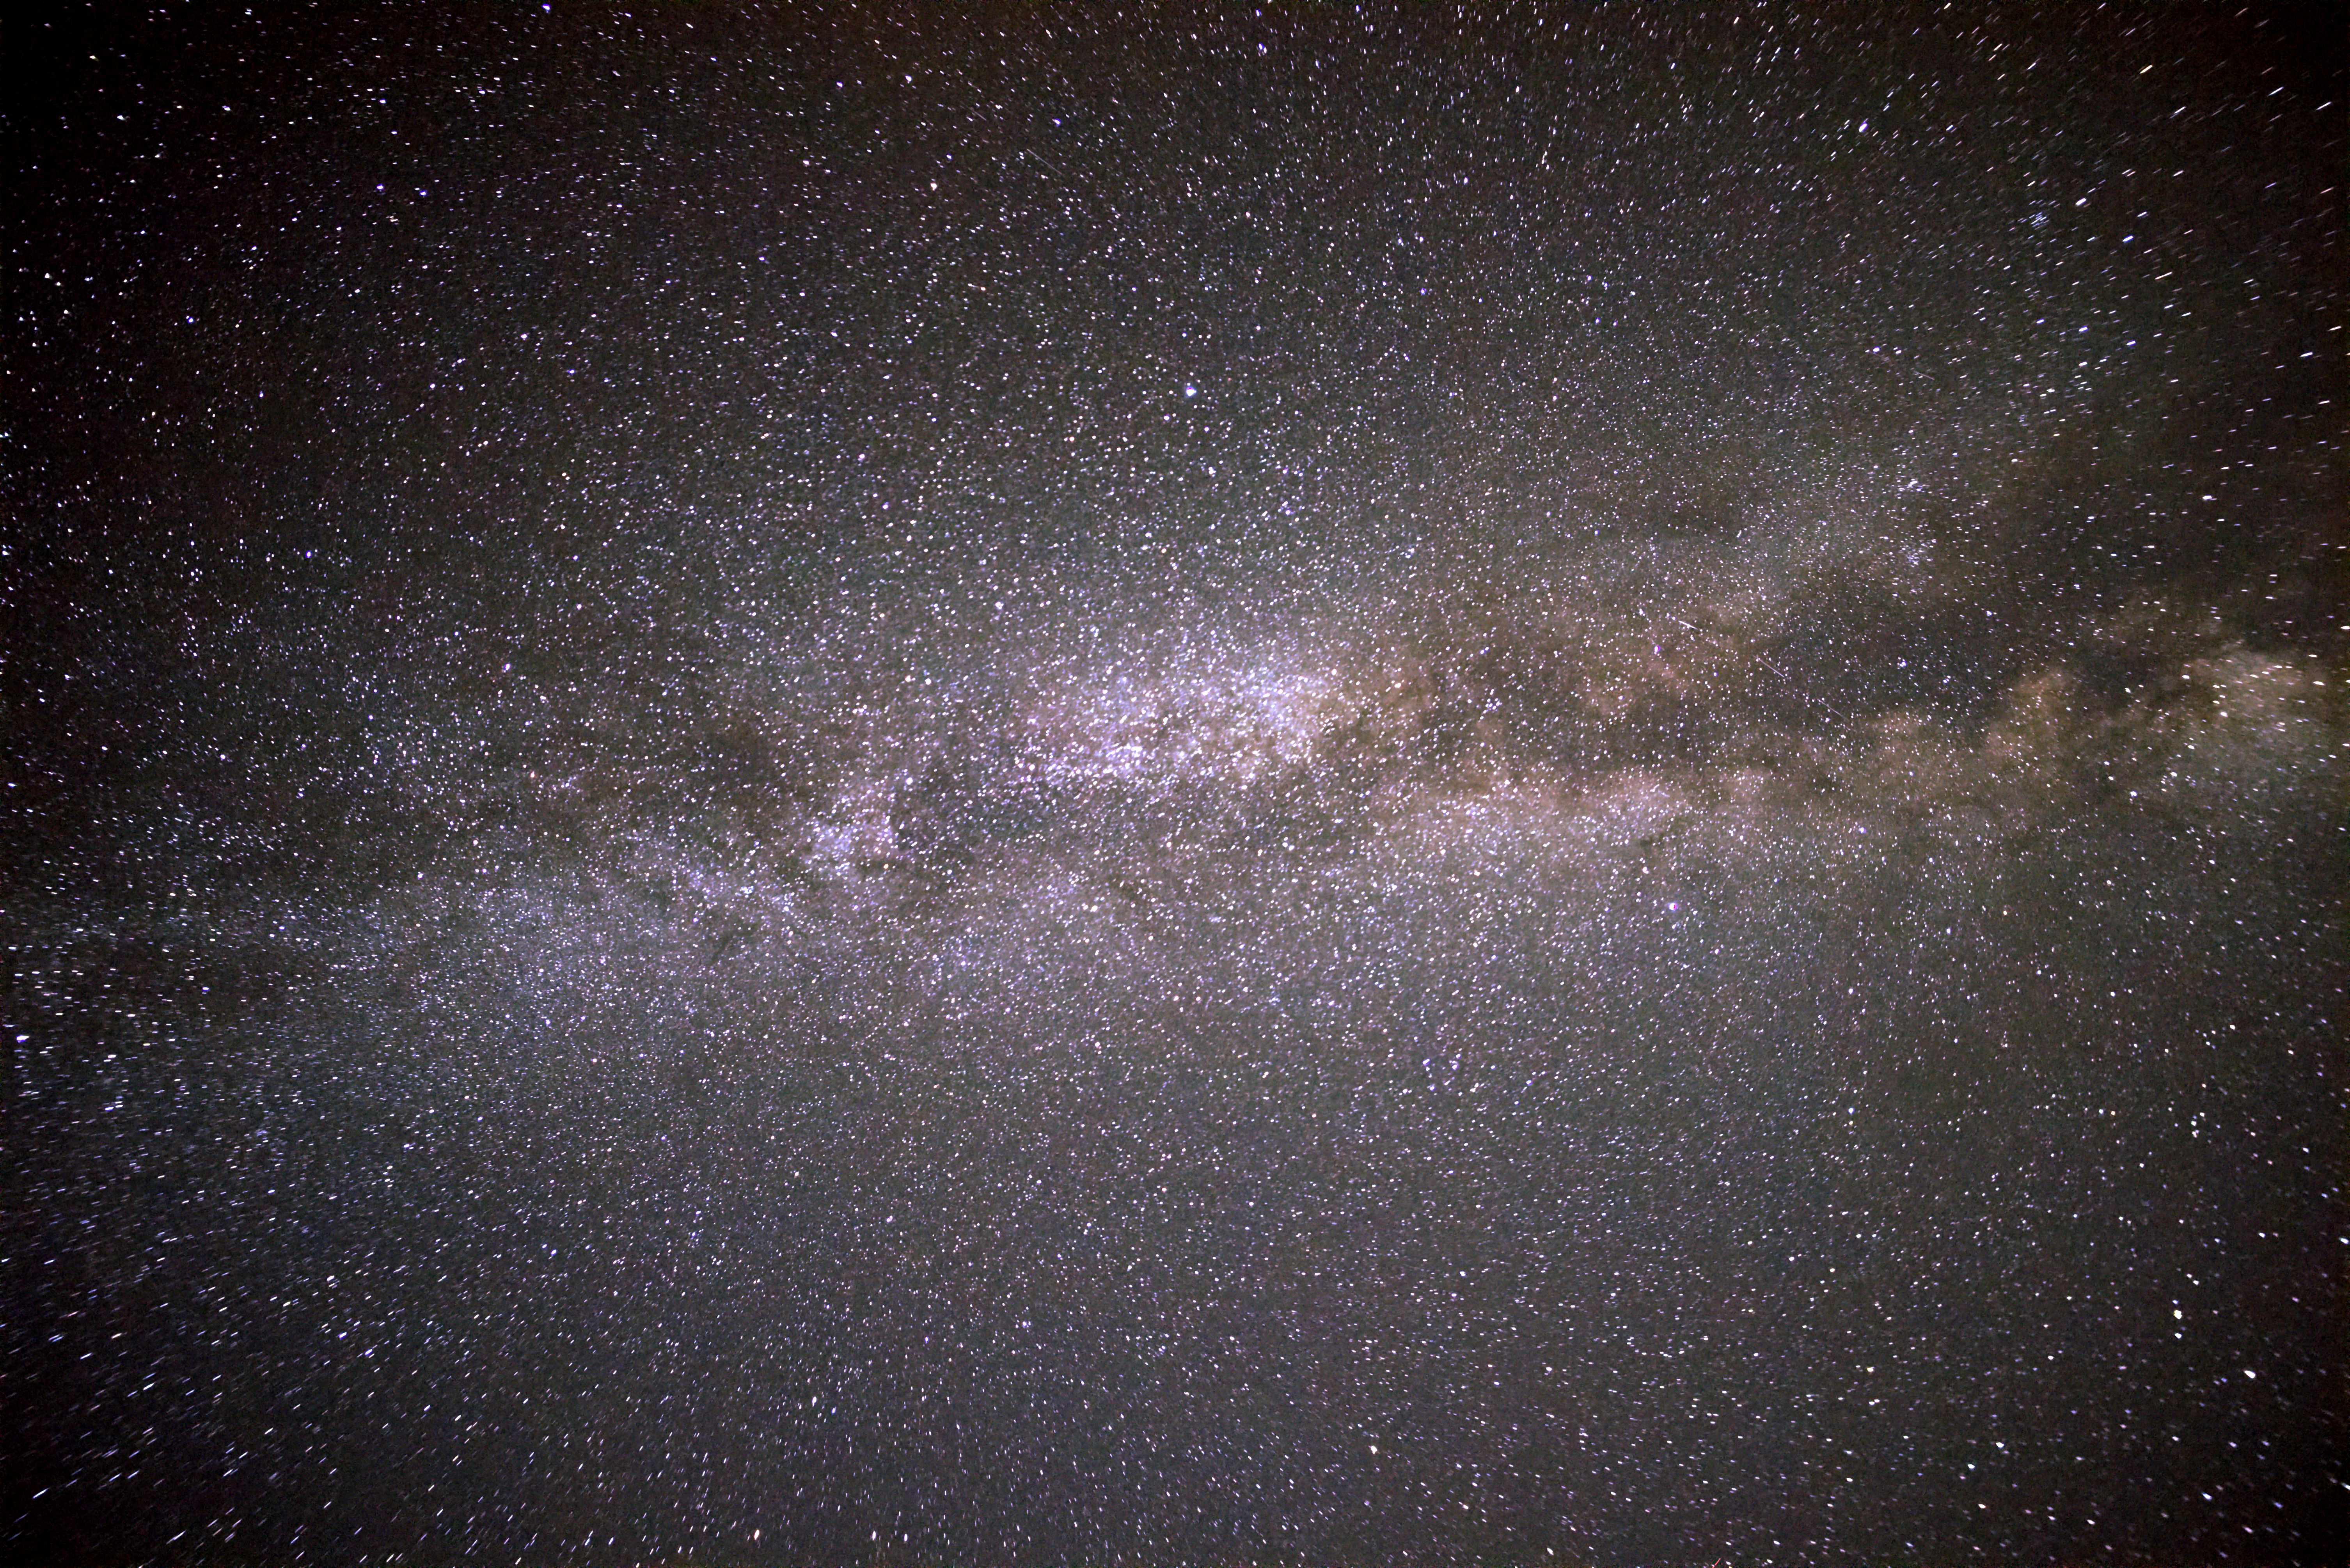
\includegraphics[width=0.7\linewidth]{sections/mori/amanogawa_okuhotaka.jpg}
  \caption{天の川}
\end{figure}

\vspace{0.5cm}

星用のカメラフィルターを持ってきたのに付け忘れてしまいました。また、キャンプ地から離れると暗くて怖すぎたのと、あまり下見できていなかったことから涸沢小屋の近くで撮影しました。そのため、小屋からの明かりを霧が反射して写真が若干明るくなってしまったように感じます。小屋の電気が消える21時以降も観測を続けたかったですが、曇ってしまったことと翌日の行動もあるため就寝しました。

\section{最後に}

泊りの登山で初めて天体観測をして、改善点などがいろいろと分かりました。

\begin{itemize}
  \item 双眼鏡を持ってくる
  \item 余裕の持った日程にして深夜まで天体観測できるようにする
  \item 小屋やテントの明かりが入らないところを下見しておく
\end{itemize}

また、涸沢は移動距離が長いので望遠鏡や赤道儀を持ち込んでの天体観測はなかなか厳しいものがあると感じました。持っていくとしてもポータブル赤道儀など、重さを減らす努力をするか、相当体力をつける必要があると思います。

天体写真撮影は機材の持ち込みが難しいという障害があるものの、星景写真を撮ることに関しては山も一緒に写すことができるので登山ととても相性がいいと感じました。尾根の上に泊まって雲海と星空を撮影したりするのも面白いと思います。


\end{document}